\documentclass[11pt,a4paper]{article}
\usepackage[margin=2.5cm]{geometry}
\usepackage{graphicx}
\usepackage{booktabs}
\usepackage{enumitem}
\usepackage{float}
\usepackage{hyperref}
\usepackage{xcolor}
\definecolor{paf}{RGB}{0,90,170}
\hypersetup{colorlinks=true,linkcolor=paf,urlcolor=paf,citecolor=paf}
\setlength{\parskip}{0.5em}
\setlength{\parindent}{0pt}

\begin{document}

% ---------------- Title page ----------------
\begin{titlepage}
\centering

\includegraphics[width=0.85\textwidth]{logo_full.png}\par
\vspace{2cm}
{\Large \textbf{Natural Language Processing}\par}
\vspace{0.5cm}
{\large Final Project Report\par}
\vspace{1.5cm}
\rule{\textwidth}{1pt}\par\vspace{0.4cm}
{\LARGE \bfseries \color{paf} Benchmarking Byte-Pair Encoding (BPE) vs.\ WordPiece
on Non-Standardized Romanized Scripts: A Roman Urdu Case Study\par}
\vspace{0.4cm}\rule{\textwidth}{1pt}\par
\vspace{2cm}
{\large \textbf{Group Members}\par}
\vspace{0.4cm}
\begin{tabular}{ll}
\toprule
\textbf{Name} & \textbf{Registration No.} \\
\midrule
Qazi Absaar Baseer Ud Din & B23F0054CS069 \\
Rania Khan               & B23F0082CS073 \\
Memmona Shafiq           & B23F0555CS086 \\
\bottomrule
\end{tabular}\par
\vfill
{\large Department of Computer Science\\
Pak-Austria Fachhochschule: Institute of Applied Sciences and Technology\par}
\vspace{0.3cm}
{\large \today\par}
\end{titlepage}

\begin{abstract}
Roman Urdu has no standard spelling, so one word appears in many written forms. We compare two subword tokenization algorithms, Byte-Pair Encoding (BPE) and WordPiece, on 19{,}489 Roman Urdu social media sentences. We train each algorithm at four vocabulary sizes (1k, 4k, 8k and 16k) and measure unknown-token rate, fertility, spelling-variant consistency and downstream sentiment classification performance. BPE produces slightly fewer tokens per word than WordPiece at every vocabulary size. Neither algorithm produces unknown tokens on the cleaned text. Both algorithms split spelling variants inconsistently, and consistency falls as the vocabulary grows, because frequent variants become separate whole-word tokens. Downstream, the best subword tokenizers (WordPiece-4k: 63.37 macro F1; BPE-16k: 63.26) perform about the same as a plain word-level baseline (63.13). For Roman Urdu, the choice between BPE and WordPiece matters less than the vocabulary size, and subword tokenization alone does not solve spelling variation.
\end{abstract}

\section{Introduction}
Roman Urdu is Urdu written in the Latin script. It is common on social media and in chat applications, but it has no standard spelling. For example, ``no'' appears as \textit{nahi}, \textit{nahin}, \textit{nai} and \textit{nhi}. This variation makes the vocabulary large and sparse.

Subword tokenizers split rare words into smaller, frequent pieces. The two most common algorithms are BPE~\cite{sennrich2016} and WordPiece~\cite{schuster2012}. BERT uses WordPiece~\cite{devlin2019}, and GPT-style models use BPE. This project measures how these two algorithms behave on noisy Roman Urdu text. We answer four research questions:
\begin{enumerate}[label=\textbf{RQ\arabic*.},leftmargin=*]
  \item Which algorithm gives lower unknown-token rate and fertility on Roman Urdu?
  \item How does vocabulary size change the results for each algorithm?
  \item Which algorithm splits spelling variants of the same word more consistently?
  \item Do differences in tokenization affect downstream classification?
\end{enumerate}

\section{Related Work}
Sennrich et al.~\cite{sennrich2016} introduced BPE for neural machine translation. BPE starts from characters and repeatedly merges the most frequent adjacent pair. Schuster and Nakajima~\cite{schuster2012} introduced WordPiece. WordPiece also merges pairs, but it picks the merge that most increases the likelihood of the training data. Kudo and Richardson~\cite{kudo2018} released SentencePiece, a language-independent toolkit for subword tokenization. Rust et al.~\cite{rust2021} showed that tokenizer quality, measured with fertility and the proportion of continued words, affects the performance of multilingual models. We use their metrics in this study. Sharf~\cite{sharf2018} released the Roman Urdu dataset that we use.

\section{Dataset}
We use the UCI Roman Urdu Data Set~\cite{sharf2018}. The raw file has 20{,}229 sentences. We apply light cleaning so that the natural spelling noise stays in the data:
\begin{itemize}[leftmargin=*]
  \item Convert text to lowercase.
  \item Remove URLs, user mentions and non-ASCII characters such as emojis.
  \item Remove empty and duplicate sentences.
  \item Fix one mislabeled class name (\texttt{Neative} to \texttt{Negative}).
\end{itemize}
After cleaning, 19{,}489 sentences remain. We use a stratified 80/20 split (random seed 42). Table~\ref{tab:data} shows the class distribution.

\begin{table}[H]
\centering
\begin{tabular}{lrrrr}
\toprule
 & \textbf{Neutral} & \textbf{Positive} & \textbf{Negative} & \textbf{Total} \\
\midrule
All sentences & 8{,}428 & 5{,}829 & 5{,}232 & 19{,}489 \\
Train (80\%) & & & & 15{,}591 \\
Test (20\%) & & & & 3{,}898 \\
\bottomrule
\end{tabular}
\caption{Dataset after cleaning.}
\label{tab:data}
\end{table}

\section{Method}
\subsection{Tokenizer Training}
We use the HuggingFace \texttt{tokenizers} library. For BPE and for WordPiece we train tokenizers with vocabulary sizes of 1k, 4k, 8k and 16k on the training split. This gives 8 tokenizers. All of them use the same whitespace pre-tokenizer, so the algorithm and the vocabulary size are the only differences.

\subsection{Intrinsic Metrics}
Each tokenizer is applied to the test split. We compute:
\begin{itemize}[leftmargin=*]
  \item \textbf{Unknown-token rate:} the percentage of tokens that are \texttt{[UNK]}.
  \item \textbf{Fertility:} the average number of tokens per word~\cite{rust2021}.
  \item \textbf{Continued words:} the percentage of words split into two or more tokens~\cite{rust2021}.
  \item \textbf{Characters per token:} the average token length, without the WordPiece \texttt{\#\#} prefix.
\end{itemize}

\subsection{Spelling-Variant Consistency}
We list 16 common Roman Urdu words with 3 or 4 spelling variants each (for example \textit{kya / kia / kyaa} and \textit{nahi / nahin / nai / nhi}). For each group we tokenize every variant and compute the Jaccard similarity of the token sets for every pair of variants. The \texttt{\#\#} prefix is removed first so that BPE and WordPiece are compared fairly. The score of a tokenizer is the mean over all groups. A higher score means the variants share more pieces.

\subsection{Downstream Classification}
For each tokenizer we convert sentences to subword tokens and train a TF-IDF and Logistic Regression sentiment classifier with \texttt{scikit-learn}. We report accuracy and macro F1-score on the test split. As a baseline we use the same classifier on plain word-level TF-IDF features.

\section{Results}
\subsection{Intrinsic Metrics}
Table~\ref{tab:intrinsic} and Figure~\ref{fig:intrinsic} show the intrinsic metrics.

\begin{table}[H]
\centering
\begin{tabular}{llrrrr}
\toprule
\textbf{Algorithm} & \textbf{Vocab} & \textbf{UNK (\%)} & \textbf{Fertility} & \textbf{Continued (\%)} & \textbf{Chars/token} \\
\midrule
BPE       & 1k  & 0.0 & 1.685 & 43.33 & 2.347 \\
BPE       & 4k  & 0.0 & 1.319 & 23.59 & 2.998 \\
BPE       & 8k  & 0.0 & 1.201 & 15.77 & 3.293 \\
BPE       & 16k & 0.0 & \textbf{1.127} & \textbf{10.31} & \textbf{3.508} \\
\midrule
WordPiece & 1k  & 0.0 & 1.807 & 47.44 & 2.189 \\
WordPiece & 4k  & 0.0 & 1.365 & 25.97 & 2.898 \\
WordPiece & 8k  & 0.0 & 1.226 & 17.26 & 3.226 \\
WordPiece & 16k & 0.0 & 1.142 & 11.41 & 3.464 \\
\bottomrule
\end{tabular}
\caption{Intrinsic metrics on the test split. Lower fertility and fewer continued words mean less fragmentation.}
\label{tab:intrinsic}
\end{table}

\begin{figure}[H]
\centering
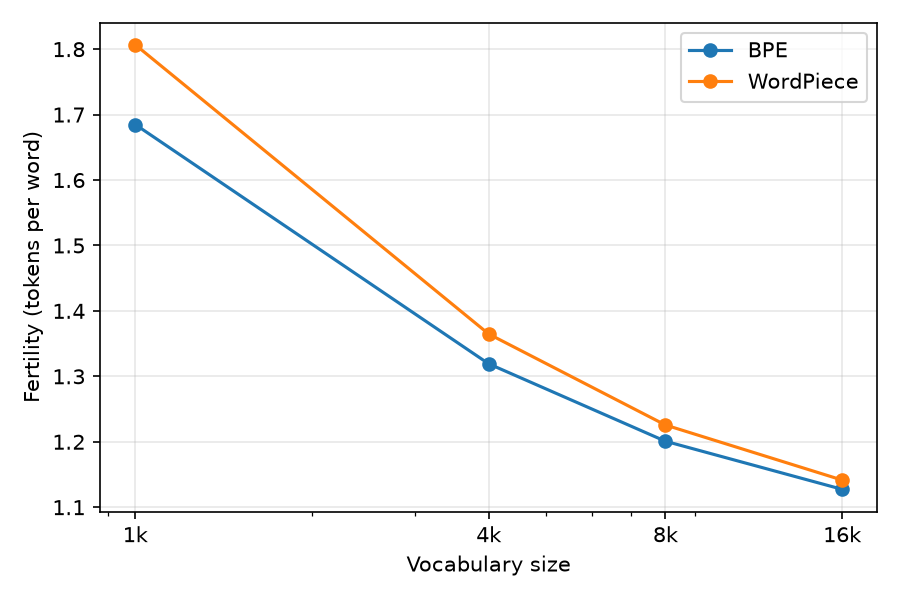
\includegraphics[width=0.49\textwidth]{results/fertility.png}
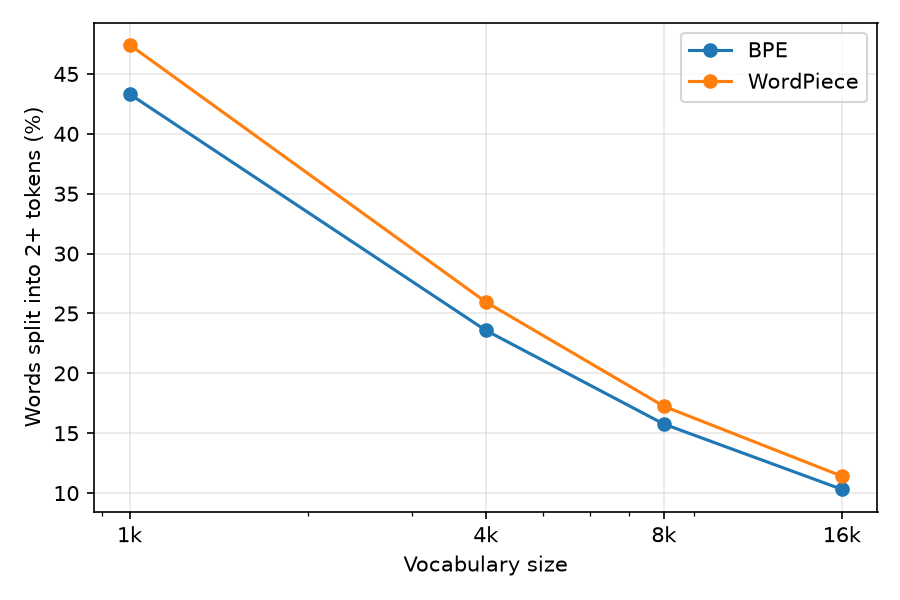
\includegraphics[width=0.49\textwidth]{results/continued_words.png}
\caption{Fertility (left) and percentage of words split into two or more tokens (right) against vocabulary size. The unknown-token rate is 0 for every tokenizer and is not plotted.}
\label{fig:intrinsic}
\end{figure}

\subsection{Spelling-Variant Consistency}
Table~\ref{tab:variants} shows the mean consistency and selected word groups. Figure~\ref{fig:variants} shows the mean against vocabulary size.

\begin{table}[H]
\centering
\begin{tabular}{lrrrrrrrr}
\toprule
 & \multicolumn{4}{c}{\textbf{BPE}} & \multicolumn{4}{c}{\textbf{WordPiece}} \\
\cmidrule(lr){2-5}\cmidrule(lr){6-9}
\textbf{Group} & 1k & 4k & 8k & 16k & 1k & 4k & 8k & 16k \\
\midrule
no (\textit{nahi, nahin, nai, nhi})  & 0.00 & 0.00 & 0.00 & 0.00 & 0.08 & 0.00 & 0.00 & 0.00 \\
happy (\textit{khush, khus, kush})   & 0.00 & 0.00 & 0.00 & 0.00 & 0.22 & 0.00 & 0.00 & 0.00 \\
fine (\textit{theek, thik, theak})   & 0.11 & 0.00 & 0.00 & 0.00 & 0.17 & 0.00 & 0.00 & 0.00 \\
thanks (\textit{shukriya, shukria, shukriyah}) & 0.55 & 0.17 & 0.17 & 0.17 & 0.55 & 0.17 & 0.17 & 0.17 \\
\midrule
\textbf{Mean (16 groups)} & 0.10 & 0.07 & 0.06 & 0.05 & \textbf{0.14} & 0.07 & 0.07 & 0.06 \\
\bottomrule
\end{tabular}
\caption{Spelling-variant consistency (mean pairwise Jaccard). Full results are in \texttt{results/variants.csv}.}
\label{tab:variants}
\end{table}

\begin{figure}[H]
\centering
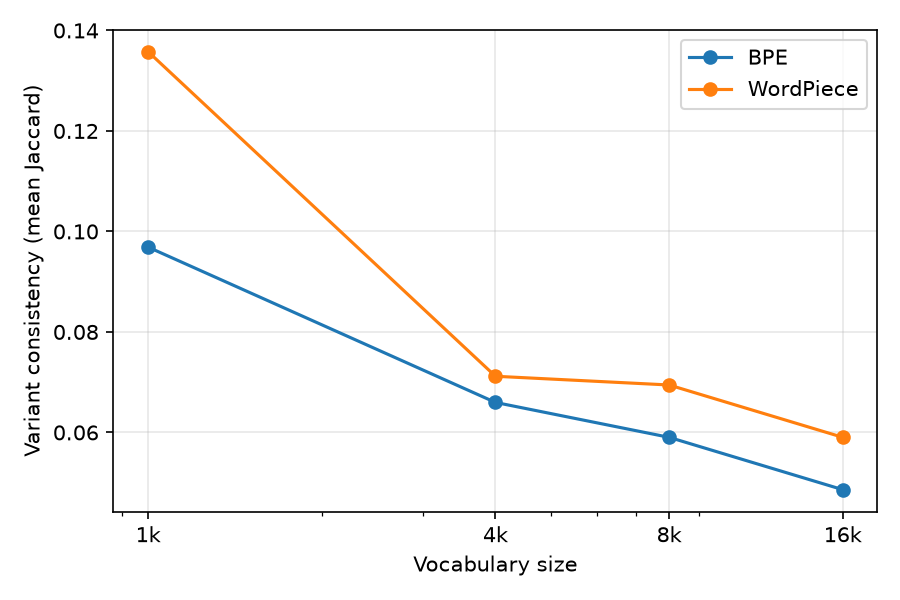
\includegraphics[width=0.6\textwidth]{results/variants.png}
\caption{Mean spelling-variant consistency against vocabulary size.}
\label{fig:variants}
\end{figure}

\subsection{Downstream Classification}
Table~\ref{tab:downstream} and Figure~\ref{fig:f1} show the sentiment classification results.

\begin{table}[H]
\centering
\begin{tabular}{llrr}
\toprule
\textbf{Tokenizer} & \textbf{Vocab} & \textbf{Accuracy (\%)} & \textbf{Macro F1 (\%)} \\
\midrule
BPE       & 1k  & 61.01 & 58.95 \\
BPE       & 4k  & 64.52 & 63.01 \\
BPE       & 8k  & 64.26 & 62.59 \\
BPE       & 16k & \textbf{65.01} & 63.26 \\
\midrule
WordPiece & 1k  & 61.06 & 58.98 \\
WordPiece & 4k  & 64.91 & \textbf{63.37} \\
WordPiece & 8k  & 64.78 & 63.07 \\
WordPiece & 16k & 64.39 & 62.63 \\
\midrule
Word-level baseline & -- & 64.78 & 63.13 \\
\bottomrule
\end{tabular}
\caption{Sentiment classification with TF-IDF and Logistic Regression on the test split.}
\label{tab:downstream}
\end{table}

\begin{figure}[H]
\centering
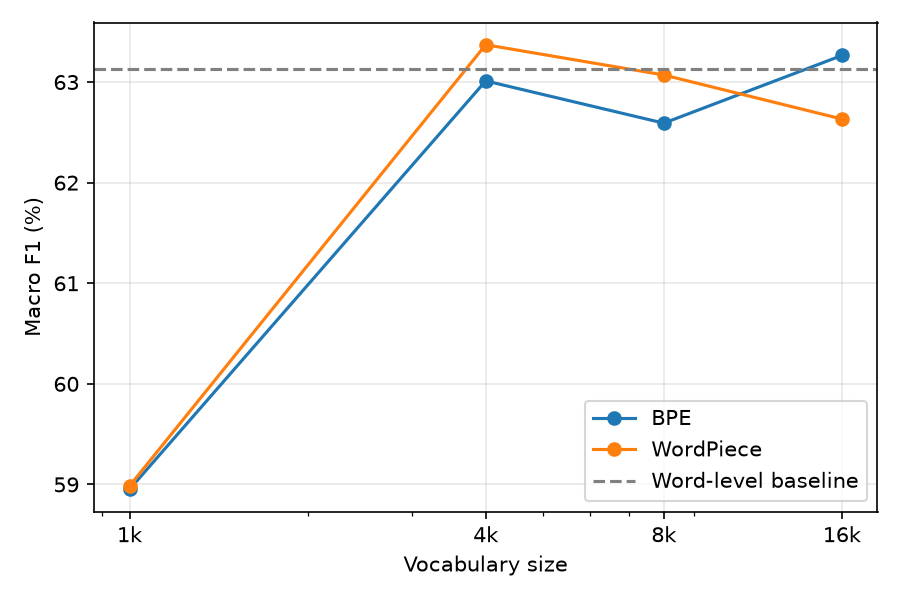
\includegraphics[width=0.6\textwidth]{results/macro_f1.png}
\caption{Macro F1 against vocabulary size. The dashed line is the word-level baseline.}
\label{fig:f1}
\end{figure}

\section{Discussion}
\textbf{RQ1 (unknown tokens and fertility).} Neither algorithm produced unknown tokens. After cleaning, the text contains only ASCII characters, and every character appears in the training data, so any word can be built from known pieces. BPE has lower fertility than WordPiece at every vocabulary size (for example 1.685 vs.\ 1.807 at 1k and 1.127 vs.\ 1.142 at 16k). BPE also splits fewer words and produces longer tokens. The gap is largest at small vocabulary sizes and almost disappears at 16k.

\textbf{RQ2 (vocabulary size).} Vocabulary size has a much bigger effect than the algorithm. Going from 1k to 16k cuts the share of split words from about 45\% to about 11\% for both algorithms. At 16k most common words, including many spelling variants, become single tokens.

\textbf{RQ3 (spelling variants).} Both algorithms handle spelling variants poorly. Mean consistency is low (0.05 to 0.14) and falls as the vocabulary grows. The reason is that frequent variants such as \textit{nahi}, \textit{nahin}, \textit{nai} and \textit{nhi} each become their own whole-word token, so they share no pieces at all. WordPiece is slightly more consistent at 1k (0.14 vs.\ 0.10) because it splits more often, which leaves more shared pieces such as \textit{nahi} + \textit{\#\#n}. At larger sizes the two algorithms are almost the same. Subword tokenization alone therefore does not group spelling variants. A normalization step, such as phonetic or edit-distance normalization, would be needed for that.

\textbf{RQ4 (downstream effect).} The 1k tokenizers are clearly worse (about 59 macro F1), because short pieces carry less meaning. From 4k upward all tokenizers score between 62.6 and 63.4 macro F1, which is close to the word-level baseline (63.13). The best result is WordPiece-4k (63.37), but the differences between the 4k--16k tokenizers are small and come from one train/test split, so we do not treat them as significant.

\textbf{Limitations.} We use one dataset, one random split and a simple linear classifier. The spelling-variant list is small and hand-made. WordPiece training in the \texttt{tokenizers} library is not fully deterministic: repeated runs change its macro F1 by up to about 0.15 points. BPE training gives identical results on every run. Results with transformer models may differ.

\section{Conclusion}
On Roman Urdu, BPE gives slightly less fragmented tokenization than WordPiece, but the difference is small compared with the effect of vocabulary size. A vocabulary of 4k to 8k tokens is a good choice: it reaches baseline-level downstream performance with a compact vocabulary. Neither algorithm groups spelling variants, so Roman Urdu pipelines should combine subword tokenization with a spelling normalization step. Future work could test transformer models, more datasets and normalization before tokenization.

All code and results are available at:\\ \url{https://github.com/QaziAbsaar/roman-urdu-subword-tokenizers}.

\begin{thebibliography}{9}
\bibitem{sennrich2016}
R.~Sennrich, B.~Haddow, and A.~Birch, ``Neural machine translation of rare words with subword units,'' in \textit{Proc.\ ACL}, 2016, pp.~1715--1725.

\bibitem{schuster2012}
M.~Schuster and K.~Nakajima, ``Japanese and Korean voice search,'' in \textit{Proc.\ IEEE ICASSP}, 2012, pp.~5149--5152.

\bibitem{devlin2019}
J.~Devlin, M.-W.~Chang, K.~Lee, and K.~Toutanova, ``BERT: Pre-training of deep bidirectional transformers for language understanding,'' in \textit{Proc.\ NAACL-HLT}, 2019, pp.~4171--4186.

\bibitem{rust2021}
P.~Rust, J.~Pfeiffer, I.~Vuli\'c, S.~Ruder, and I.~Gurevych, ``How good is your tokenizer? On the monolingual performance of multilingual language models,'' in \textit{Proc.\ ACL-IJCNLP}, 2021, pp.~3118--3135.

\bibitem{kudo2018}
T.~Kudo and J.~Richardson, ``SentencePiece: A simple and language independent subword tokenizer and detokenizer for neural text processing,'' in \textit{Proc.\ EMNLP: System Demonstrations}, 2018, pp.~66--71.

\bibitem{sharf2018}
Z.~Sharf, ``Roman Urdu Data Set,'' UCI Machine Learning Repository, 2018. \url{https://archive.ics.uci.edu/dataset/458/roman+urdu+data+set}
\end{thebibliography}

\end{document}
